\documentclass[12pt]{article}
\usepackage[english]{babel}
\usepackage[utf8]{inputenc}
\usepackage{amsmath, amssymb, amsthm}
\usepackage{graphicx}
\usepackage{hyperref}
\usepackage[margin=.75in]{geometry}
\usepackage{xcolor}
\usepackage{tikz}

\newcommand{\id}{\text{id}}
\newcommand{\od}{\text{od}}

\setlength{\topmargin}{0pt}
\setlength{\headsep}{0pt}
\textheight = 600pt

\title{Graph Theory \\ Homework 11}
\author{Ben Kallus and Ryan Friedman}
\date{Due Friday, April 2}

\begin{document}
\maketitle

\noindent\textbf{7.8} Proposition: If every vertex of some tournament of order $n$ has the same outdegree $x$, then $x = \frac{n-1}2$.
\begin{proof}
	Let $T$ be a tournament of order $n$ such that each vertex in $V(T)$ has outdegree $x$.
	Then, since a tournament has $\frac{n(n-1)}2$ arcs, and each arc contributes 1 to the total outdegree of the graph, $$nx = \frac{n(n-1)}2.$$
	Thus, $$x = \frac{n-1}2.$$
\end{proof}

\newpage\noindent\textbf{7.10} Proposition: If $u$ and $v$ are vertices of a tournament such that $\vec{d}(u,v) = k$, then $\id(u) \geq k - 1$.
\begin{proof}
	Let $T$ be a tournament, and let $u,v \in V(T)$ such that $\vec d(u,v) = k$.
	Then, the shortest directed $u-v$ path $P = (u = p_0, \hdots, p_k = v)$ has length $k$.
	Since $P$ is the shortest $u-v$ path, it must be that $p_1u, p_2u, \hdots, p_ku \in A(T)$.
	Thus, $\id(u) \geq k-1$.
\end{proof}
	

\newpage\noindent\textbf{7.12}

\textbf{(a)} Proposition: If every vertex in a tournament $T$ belongs to a cycle in $T$, then $T$ is not necessarily strong.
\begin{proof}
	Begin constructing a graph $G$ with $C_3 \cup C_3$.
	Then, orient each cycle such that each vertex has indegree 1 and outdegree 1.
	Then, add all possible arcs from vertices in the first cycle to vertices in the second cycle.

	Note that every vertex in $G$ belongs to one of the original cycles from which it was constructed, but there is no directed path from a vertex in the second cycle to a vertex in the first.
\end{proof}

\textbf{(b)} Proposition: For every pair $u,v$ of vertices in a strong tournament $T$, there may exist neither a Hamiltonian $u-v$ path nor a Hamiltonian $v-u$ path.
\begin{proof}
	Consider the following directed graph $G$:
	\begin{center}\includegraphics[angle=90]{712b.png}\end{center}

	A $u-v$ Hamiltonian path must visit $v$ last, so it must begin with $u$ followed by $x$.
	Note that the vertex after $x$ cannot be $y$, because its only outward edge leads to $u$, which would leave $v$ unvisited.
	Now, observe that the vertex after $x$ cannot be $v$, because $v$ must be the last vertex in the path, so $y$ would be unvisited.
	Therefore, $G$ has no $u-v$ Hamiltonian path.
	
	A $v-u$ Hamiltonian path must visit $u$ last, so it must begin with $v$ followed by $y$.
	The vertex after $y$ must be $u$, since $y$ has a single outward edge, but that would leave $x$ unvisited.
	Therefore, $G$ has no $v-u$ Hamiltonian path.
\end{proof}

\textbf{(c)} If $(u,v)$ is an arc of a strong tournament $T$, then $(u,v)$ may not lie on a Hamiltonian cycle of $T$.
\begin{proof}
	Consider the graph $G$ from \textbf{(b)}.
	Suppose that the arc $(u,v)$ were in a Hamiltonian cycle of $G$.
	Then, since there is no directed path from $v$ to $x$ that does not pass through $x$, it must be that $x$ is not in our Hamiltonian cycle, which is a constradiction.
	Thus, $(u,v)$ participates in no Hamiltonian cycle of $G$.
\end{proof}

\newpage\noindent\textbf{7.14}

\textbf{(a)} Proposition: If an odd number of teams play in a round robin tournament, it is possible for all teams to tie for first place.
\begin{proof}
	Consider the graph $K_n$, for any odd $n \geq 1$.
	Each vertex in $K_n$ has even degree.
	Thus, $K_n$ is Eulerian by Theorem 6.1.
	Therefore, by the result of Exercise 7.2, $K_n$ has an Eulerian orientation $E$.
	Observe that in $E$, each vertex in $K_n$ has equal indegree and outdegree.
	Thus, $E$ is a tournament representing a round robin in which all teams tie for first place.
\end{proof}


\textbf{(b)} Proposition: If an even number of teams play in a round robin tournament, then it is not possible for all teams to tie for first place.
\begin{proof}
	Let $T$ be a tournament of even order $n$ representing a round robin in which all teams had the same number of victories.
	Then, all vertices in $T$ have the same outdegree $x$.
	Then, $m$, the number of arcs in $T$, is equal to $xn$.
	Because $T$ is a tournament, it has $\frac{n(n-1)}2$ arcs.
	Thus, $\frac{n(n-1)}2 = xn$, so $\frac{n-1}2 = x$.
	However, since $n$ is even, $\frac{n-1}2$ is not an integer.
	However, $x$ must be an integer, so it must be that it is not possible for all vertices in $T$ to have the same outdegree.
\end{proof}


\newpage\noindent\textbf{8.1}

\noindent\textbf{(a)}
\begin{center}
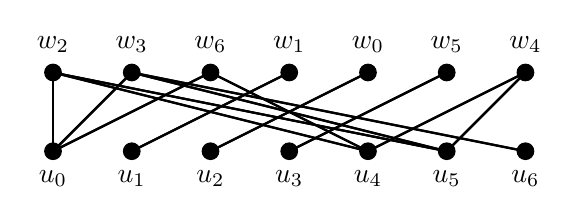
\begin{tikzpicture}
\draw[fill=black] (0, 0) circle (3pt);
\node at (0, -0.35) {$u_0$};
\draw[fill=black] (0, 1) circle (3pt);
\node at (0, 1.35) {$w_2$};
\draw[fill=black] (1, 1) circle (3pt);
\node at (1, 1.35) {$w_3$};
\draw[fill=black] (2, 1) circle (3pt);
\node at (2, 1.35) {$w_6$};
\draw[fill=black] (1, 0) circle (3pt);
\node at (1, -0.35) {$u_1$};
\draw[fill=black] (3, 1) circle (3pt);
\node at (3, 1.35) {$w_1$};
\draw[fill=black] (2, 0) circle (3pt);
\node at (2, -0.35) {$u_2$};
\draw[fill=black] (4, 1) circle (3pt);
\node at (4, 1.35) {$w_0$};
\draw[fill=black] (3, 0) circle (3pt);
\node at (3, -0.35) {$u_3$};
\draw[fill=black] (5, 1) circle (3pt);
\node at (5, 1.35) {$w_5$};
\draw[fill=black] (4, 0) circle (3pt);
\node at (4, -0.35) {$u_4$};
\draw[fill=black] (6, 1) circle (3pt);
\node at (6, 1.35) {$w_4$};
\draw[fill=black] (5, 0) circle (3pt);
\node at (5, -0.35) {$u_5$};
\draw[fill=black] (6, 0) circle (3pt);
\node at (6, -0.35) {$u_6$};

\draw[thick] (0, 0) -- (0, 1);
\draw[thick] (0, 0) -- (2, 1);
\draw[thick] (0, 0) -- (1, 1);
\draw[thick] (0, 1) -- (4, 0);
\draw[thick] (0, 1) -- (0, 0);
\draw[thick] (0, 1) -- (5, 0);
\draw[thick] (1, 1) -- (0, 0);
\draw[thick] (1, 1) -- (6, 0);
\draw[thick] (1, 1) -- (5, 0);
\draw[thick] (2, 1) -- (4, 0);
\draw[thick] (2, 1) -- (0, 0);
\draw[thick] (1, 0) -- (3, 1);
\draw[thick] (3, 1) -- (1, 0);
\draw[thick] (2, 0) -- (4, 1);
\draw[thick] (4, 1) -- (2, 0);
\draw[thick] (3, 0) -- (5, 1);
\draw[thick] (5, 1) -- (3, 0);
\draw[thick] (4, 0) -- (0, 1);
\draw[thick] (4, 0) -- (2, 1);
\draw[thick] (4, 0) -- (6, 1);
\draw[thick] (6, 1) -- (4, 0);
\draw[thick] (6, 1) -- (5, 0);
\draw[thick] (5, 0) -- (0, 1);
\draw[thick] (5, 0) -- (1, 1);
\draw[thick] (5, 0) -- (6, 1);
\draw[thick] (6, 0) -- (1, 1);
\end{tikzpicture}
\end{center}

\noindent\textbf{(b)}

	$G$ contains the perfect matching $$\{u_2w_0, u_3w_5, u_6w_3, u_1w_1, u_0w_6, u_4w_2, u_5w_4\}.$$

\newpage\noindent\textbf{8.2}

\noindent\textbf{(a)} \begin{center}\includegraphics[angle=90,scale=.5]{82a.png}\end{center}

\noindent\textbf{(b)} It is not possible to hire all six applicants for six different positions beacuse Alvin, Connie, Edward, and Frances are four applicants applying for only three different jobs, so at least one of them cannot be hired.

\newpage\noindent\textbf{8.4} Proposition: If a connected bipartite graph $G$ with partite sets $U, W$ satisfying $|U| = |W| \geq 2$, and every two vertices of $U$ have distinct degrees, then $G$ has a perfect matching.
\begin{proof}
	Let $G$ be a connected, bipartite graph of order $2k$ with partite sets $U$ and $W$ of equal order $k \geq 2$.
	Note that since $G$ is connected and nontrivial, it contains no vertices of degree 0.
	Suppose that every two vertices of $U$ have distinct degrees.
	Let $X \subseteq U$.
	Then, $|X| = j \leq k$.
	Since each vertex in $U$ has distinct degree, and $G$ contains no vertices of degree 0, the vertex of maximum degree in $U$ must have degree at least $j$.
	Thus, $|N(X)| \geq j = |X|$, so Hall's condition is satisfied.
	Thus, by Hall's Matching Theorem, $G$ has a matching of size $|U| = k$.
	This matching is perfect, because its size is equal to $\frac{|V(G)|}{2}$.
\end{proof}
	
\newpage\noindent\textbf{ALSO}

\noindent\textbf{(1)} Proposition: For any bipartite graph $G$, $\partial(G) \geq 0$.
\begin{proof}
	Let $G$ be a bipartite graph with partite sets $U,W$ satisfying $|U| \leq |W|$.
	Then, since $\emptyset \subseteq U$, and $\partial(\emptyset) = |\emptyset| - |\emptyset| = 0$, $\max\{\partial(X) \mid X \subseteq U\} \geq 0$.
	Thus, $\partial(G) \geq 0$.
\end{proof}

\noindent\textbf{(2)} Proposition: $G$ has a matching of size $|U|$ if and only if $\partial(G) = 0$.
\begin{proof}
	Let $G$ be a bipartite graph with partite sets $U,W$ satisfying $|U| \leq |W|$.
	
	Suppose that $G$ has a matching of size $|U|$.
	Then, by Hall's Matching Theorem, $G$ satisfies Hall's condition.
	Thus, $|X| \leq |N(X)|$ for all $X \subseteq U$.
	Therefore, $|X| - |N(X)| \leq 0$ for all $X \subseteq U$.
	Thus, by \textbf{(1)}, $\partial(G) = 0$.

	Now, suppose that $\partial(G) = 0$.
	Then, for all $X \subseteq U, |X| - |N(X)| \leq 0$.
	Therefore, $|X| \leq |N(X)|$.
	Thus, by Hall's Matching Theorem, $G$ has a matching of size $|U|$.
\end{proof}

\noindent\textbf{(3)} Proposition: The size of a maximum matching of $G$ is $|U| - \partial(G)$.
\begin{proof}
	Let $G$ be a bipartite graph with partite sets $U,W$ satisfying $|U| \leq |W|$.
	Consider a set $X \subseteq U$ that maximizes $|X| - \partial(X)$.
	Then, $\partial(G) = \partial(X)$.
	Create a new bipartite graph $G^*$ by adding $\partial(G)$ new vertices to $W$ and making each of them adjacent to every vertex in $U$.
	Then, since each vertex in $U$ has been affected equally by the new vertices, $X$ maximizes $|X| - \partial(X)$ in $G^*$, as well.
	Then,
	\begin{align*}
		\partial(G^*) &= |X| - |N_{G^*}(X)| \\
		              &= |X| - |N_G(X)| - \partial_G(X) \\
			      &= |X| - |N_G(X)| - (|X| - |N(X)|) \\
			      &= 0.
	\end{align*}
	Therefore, by \textbf{(2)}, $G$ has a matching of size $|U|$.
	This is a matching of maximum size, since $G$ is bipartite, so any more than $|U|$ edges in a matching would have to be incident to a vertex in $U$, and all vertices in $U$ are already covered by the original matching.
\end{proof}

\end{document}
